\documentclass[a4paper,12pt]{article}
\usepackage[indonesian]{babel}
\usepackage{graphicx}
\usepackage{multirow}
\usepackage{enumitem}
\usepackage{listings}
\usepackage{wrapfig}
\usepackage[T1]{fontenc}
\usepackage{inconsolata}
\usepackage{lipsum}
\usepackage{adjustbox}


\usepackage{color}
\usepackage[table]{xcolor}
\definecolor{mygreen}{rgb}{0,0.6,0}
\definecolor{mygray}{rgb}{0.5,0.5,0.5}
\definecolor{mymauve}{rgb}{0.58,0,0.82}
\lstset{%
    language=java,
    showstringspaces=false,          % Prevent tex replacing space to bracket in code
    frame=single,                    % Set frame around code
    backgroundcolor=\color{white},   % choose the background color
    basicstyle=\footnotesize,        % size of fonts used for the code
    breaklines=true,                 % automatic line breaking only at whitespace
    captionpos=b,                    % sets the caption-position to bottom
    commentstyle=\color{mygreen},    % comment style
    keywordstyle=\color{blue},       % keyword style
    stringstyle=\color{mymauve},     % string literal style
}

\graphicspath{ {./img/} }
\begin{document}
\title{ {\Large Laporan Praktikum}\\ Algoritma dan Pemrograman Lanjut\\{\Large Pertemuan 10}}

\author{Aldzikri Dwijayanto Prathama
    \\195410189
    \\Informatika}
\makeatletter
\begin{titlepage}
    \begin{center}
        {\huge \bfseries \@title}\\[14ex]
        
\includegraphics[scale=.8]{logo}\\[4ex]
        {\large \@author}\\[12ex]
        {\large \bfseries {SEKOLAH TINGGI MANAJEMEN INFORMATIKA DAN KOMPUTER
            AKAKOM YOGYAKARTA}}
    \end{center}


%{\large \@date}
\end{titlepage}
\makeatother
%\maketitle
\newpage
\tableofcontents
\newpage

\section{Tujuan}
Mahasiswa dapat menyelesaikan kasus dengan menggabungkan konsep iterasi, seleksi dalam method serta dapat memanngil
method dari class lain.
\section{Teori}
\paragraph{}
Pernyataan seleksi, perulangan dan fungsi sudah dibahas pada pertemuan sebelumnya.
Pada dasarnya pemakaian ketiganya dapat digabungkan dalam suatu array, data tunggal maupun data berupa array.
Untuk modul kali ini akan dipraktekkan beberapa program yang menggabungkan seleksi, perulangan dalam suatu fungsi.
\newpage

\section{Pembahasan}
\subsection{Praktik}
\subsubsection{Praktik 1}
\begin{lstlisting}
import java.util.Scanner;

public class ProyekIterasiFungsi {

    public static void cetakUlang(int nUlang) {
       
        for (int i = 0; i < nUlang; i++) {
           System.out.println("Cetak ke "+(i+1)); 
        }
    }

    public static void main(String[] args) {

        int nUlang;
        Scanner scan = new Scanner(System.in);
        System.out.print("Akan dicetak berapa kali? ");
        nUlang = scan.nextInt();
        cetakUlang(nUlang);
    }
}
\end{lstlisting}

Program tersebut memiliki du buah fungsi, fungsi cetakUlang berisi iterasi, yang berfungsi untuk mencetak bilangan ke
layar. Lalu fungsi main berfungsi untuk input, dan memanggil fungsi.

\begin{center}
    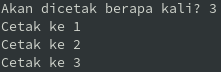
\includegraphics[scale=1]{1.png} 
\end{center}

\subsubsection{Praktik 2}
\begin{lstlisting}
import java.util.Scanner;

public class ProyekIterasiFungsia {

    public static void cetakUlang(int nUlang, String kalimat) {
       
        for (int i = 0; i < nUlang; i++) {
           System.out.println("Cetak ke "+(i+1)); 
           System.out.println(kalimat);
        }
    }

    public static void main(String[] args) {

        int nUlang;
        String kalimat;
        Scanner scan = new Scanner(System.in);
        System.out.print("Akan dicetak berapa kali? ");
        nUlang = scan.nextInt();
        scan.nextLine();
        System.out.print("Kalimat yang akan dicetak = ");
        kalimat = scan.nextLine();
        cetakUlang(nUlang,kalimat);
    }
}
\end{lstlisting}
Program tersebut memiliki dua buah fungsi, fungsi cetakUlang berisi iterasi, yang berfungsi untuk mencetak bilangan ke
layar. Lalu fungsi main berfungsi untuk input, dan memanggil fungsi. Kedua fungsi ditambahkan variabel string, untuk
menyimpan kalimat yang ingin dicetak oleh user.

\begin{center}
    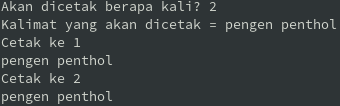
\includegraphics[scale=1]{2.png} 
\end{center}


\subsubsection{Praktik 3}
\begin{lstlisting}
import java.util.Scanner;

public class ProyekHitungJumlah {

    public static int hitungJumlah(int[] x) {
        
        int jum=0;
        for (int i=0; i<x.length; i++){
            jum += x[i];
        }
        return jum;
    }

    public static void main(String[] args) {

        int data[] = new int[10];
        int jumlah;
        Scanner scan = new Scanner(System.in);
        for (int i=0; i<10; i++){
            System.out.println("Masukkan data ke-"+(i+1)+":");
            data[i] = scan.nextInt();
        }
        jumlah = hitungJumlah(data);
        System.out.println("Jumlah data = "+jumlah);
    }
}
\end{lstlisting}
Program pada praktik 3 ini memiliki 2 buah method. Method pertama memiliki pernyataan iterasi yang berguna untuk
melakukan penjumlahan data. Sedangkan method main juga memiliki iterasi yang berguna untuk memasukkan data ke dalam
array, dan menampilkan hasil penjumlahan array.

\begin{center}
    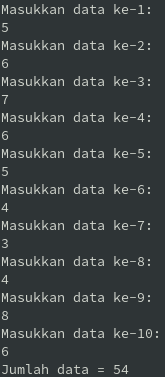
\includegraphics[scale=1]{3.png} 
\end{center}

\subsubsection{Praktik 4}
\begin{lstlisting}
import java.util.Scanner;

public class ProyekHitungJumlaha {

    public static int hitungJumlah(int[] x) {
        
        int jum=0;
        for (int i=0; i<x.length; i++){
            jum += x[i];
        }
        return jum;
    }

    public static float hitungRata(int x, int y) {

        float hasil = x/y;
        return hasil;
    }

    public static void main(String[] args) {

        int batas = 10;
        int data[] = new int[batas];
        int jumlah;
        float rata;
        Scanner scan = new Scanner(System.in);
        for (int i=0; i<10; i++){
            System.out.println("Masukkan data ke-"+(i+1)+":");
            data[i] = scan.nextInt();
        }
        jumlah = hitungJumlah(data);
        rata = hitungRata(jumlah,batas);
        System.out.println("Jumlah data = "+jumlah);
        System.out.println("Rata-rata = "+rata);
    }
}
\end{lstlisting}
Program pada praktik ini memiliki 3 buah method. Method pertama memiliki pernyataan iterasi yang berguna untuk
melakukan penjumlahan data. Method kedua berguna untuk menghitung rata-rata. Sedangkan method main memiliki iterasi
yang berguna untuk memasukkan data ke dalam array, dan menampilkan hasil penjumlahan array dan rata-rata.

\begin{center}
    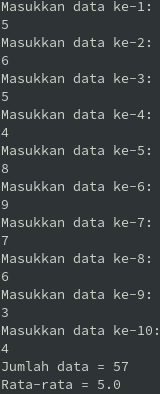
\includegraphics[scale=1]{4.png} 
\end{center}


\subsubsection{Praktik 5}
\begin{lstlisting}
import java.util.Scanner;

public class ProyekCekGenap1 {

    public static boolean cekGenap(int a) {
        boolean status;
        if ((a%2) == 0) {
            status = true;
        } else {
            status = false;
        }
        return status;
    }

    public static void main(String[] args) {

        Scanner scan = new Scanner(System.in);
        int x;
        boolean genap;
        System.out.print("Masukkan bilangan : ");
        x = scan.nextInt();
        genap = cekGenap(x);
        if (genap) {
            System.out.println("Bilangan yang dicek ternyata genap");
        } else {
            System.out.println("Bilangan yang dicek ternyata ganjil");
        }
    }
}
\end{lstlisting}

Program pada praktik 5 dua method. Method cekGenap memiliki seleksi, untuk mengecek bilangan ganjil atau genap. Jika
bilangan yang dimasukkan genap maka method mengembalikan nilai boolean true, sedangkan jika ganjil, method mengembalikan
nilai boolean false. Sedangkan pada method main, berguna untuk memasukkan nilai, dan mencetak kalimat. Jika nilai yang
didapat dari method cekGenap bernilai true, maka method main akan mencetak kalimat genap.

\begin{center}
    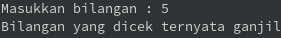
\includegraphics[]{5.png} 
\end{center}

\subsubsection{Praktik 6}
\begin{lstlisting}
import java.util.Scanner;

/**
 * ProyekCekGanjilGenapArray
 */
public class ProyekCekGanjilGenapArray {

   public static boolean[] cekGanjilGenapArray(int[] x) {
       boolean hasil[] = new boolean[10];
       for (int i=0; i<x.length; i++) {
           if ((x[i] % 2) == 0) {
               hasil[i] = true;
           } else {
               hasil[i] = false;
           }
       }
       return hasil;
   }

   public static void main(String[] args) {
       int data[] = new int[10];
       boolean hasilCek[] = new boolean[10];
       Scanner scan = new Scanner(System.in);
       for (int i=0; i<10; i++) {
           System.out.println("Masukkan data ke-"+(i+1)+":");
           data[i] = scan.nextInt();
       }
       hasilCek = cekGanjilGenapArray(data);
       System.out.println("==========================");
       System.out.println("==Hasil Pengecekan========");
       System.out.println("==========================");

       for (int i=0; i<10; i++) {
           System.out.print(" "+data[i]);
           System.out.print(" "+hasilCek[i]);
           System.out.println();
       }
   }
}
\end{lstlisting}

Program pada praktik 6 dua method. Method pertama memiliki seleksi, untuk mengecek bilangan ganjil atau genap. Jika
bilangan yang dimasukkan genap maka method mengembalikan nilai boolean true, sedangkan jika ganjil, method mengembalikan
nilai boolean false. Sedangkan pada method main, berguna untuk memasukkan nilai, dan mencetak kalimat. Jika nilai yang
didapat dari method cekGenap bernilai true, maka method main akan mencetak kalimat true.
\begin{center}
    
\includegraphics[scale=1]{6.png} 
\end{center}

\subsubsection{Praktik 7}
\begin{lstlisting}
import java.util.Scanner;

public class ProyekCekGanjilGenapArraya {

   public static boolean[] cekGanjilGenapArray(int[] x) {
       boolean hasil[] = new boolean[10];
       for (int i=0; i<x.length; i++) {
           if ((x[i] % 2) == 0) {
               hasil[i] = true;
           } else {
               hasil[i] = false;
           }
       }
       return hasil;
   }

   public static void main(String[] args) {
       int data[] = new int[10];
       boolean hasilCek[] = new boolean[10];
       Scanner scan = new Scanner(System.in);
       for (int i=0; i<10; i++) {
           System.out.println("Masukkan data ke-"+(i+1)+":");
           data[i] = scan.nextInt();
       }
       hasilCek = cekGanjilGenapArray(data);
       System.out.println("==========================");
       System.out.println("==Hasil Pengecekan========");
       System.out.println("==========================");

       for (int i=0; i<10; i++) {
           System.out.print(" "+data[i]);
           System.out.print(" "+(hasilCek[i]? "Genap":"Ganjil"));
           System.out.println();
       }
   }
}
\end{lstlisting}

Program pada praktik 7 memiliki dua method. Method pertama memiliki seleksi, untuk mengecek bilangan ganjil atau genap. Jika
bilangan yang dimasukkan genap maka method mengembalikan nilai boolean true, sedangkan jika ganjil, method mengembalikan
nilai boolean false. Sedangkan pada method main, berguna untuk memasukkan nilai, dan mencetak kalimat. Jika nilai yang
didapat dari method cekGenap bernilai true, maka method main akan mencetak kalimat genap.
\begin{center}
    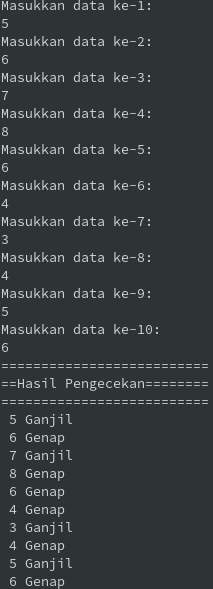
\includegraphics[scale=1]{7.png} 
\end{center}

\newpage

\subsection{Latihan}
\begin{lstlisting}
import java.util.Scanner;

public class KonversiNilai {

    public static void main(String[] args) {
		Scanner scan = new Scanner(System.in);
		double[] data = new double[10];
		char [] keluar = new char[10];
		for (int i=0;i<10;i++){
			System.out.print("data ke-"+(i+1)+":");
			data[i] = scan.nextDouble();
		}
		System.out.println("=====================");
		System.out.println("|   Hasil Konversi  |");
		System.out.println("=====================");
		keluar = konversiNilai(data);

		for (int i=0;i<10;i++){
			System.out.println(data[i]+"  "+keluar[i]);
		}
	}
	public static char[] konversiNilai(double[] x) {
		int n = x.length;
        char hasil[] = new char[n];
        for (int i = 0; i < n; i++) {
			if ((x[i] > 80) && (x[i] <= 100)) {
				hasil[i] = 'A';
			} else if ((x[i] > 60) && (x[i] <= 80)) {
				hasil[i] = 'B';
			} else if ((x[i] > 40) && (x[i] <= 60)) {
				hasil[i] = 'C';
			} else if ((x[i] > 20) && (x[i] <= 40)) {
				hasil[i] = 'D';
			} else if (x[i] <= 20) {
				hasil[i] = 'E';
			}
		}
		return hasil;
	}
}
\end{lstlisting}

Program pada Latihan, memiliki dua method, method pertama berfungsi untuk memasukkan nilai, memanggil method untuk
konversi, dan menampilkan hasil. Sedangkan method kedua berguna untuk mengkonversi nilai yang berada pada array.

\begin{center}
    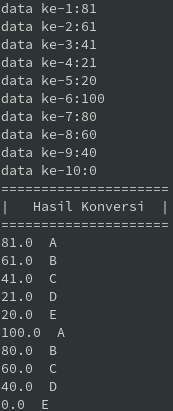
\includegraphics[scale=1]{8.png} 
\end{center}

\newpage

\subsection{Tugas}
\begin{lstlisting}
import java.util.Scanner;

public class KonversiNilai2 {

    public static void main(String[] args) {
		Scanner scan = new Scanner(System.in);
		double[] data = new double[10];
		char [] keluar = new char[10];
        int i=0;
		while (i<10){
			System.out.print("data ke-"+(i+1)+":");
			data[i] = scan.nextDouble();
            i++;
		}
		System.out.println("=====================");
		System.out.println("|   Hasil Konversi  |");
		System.out.println("=====================");
		keluar = konversiNilai(data);

        i=0;
		while (i<10){
			System.out.println(data[i]+"  "+keluar[i]);
            i++;
		}
	}
	public static char[] konversiNilai(double[] x) {
		int n = x.length;
        char hasil[] = new char[n];
        int i=0;
        while (i < n) {
        int nilai=0;
            if ((x[i] - 80) > 0) {
                nilai++;
            }
            if ((x[i] - 60) > 0) {
                nilai++;
            }
            if ((x[i] - 40) > 0) {
                nilai++;
            }
            if ((x[i] - 20) > 0) {
                nilai++;
            }
            if (x[i] <= 20) {
                nilai=0;
            }
            switch(nilai) {
                case 4:
                hasil[i] = 'A';
                break;
                case 3:
                hasil[i] = 'B';
                break;
                case 2:
                hasil[i] = 'C';
                break;
                case 1:
                hasil[i] = 'D';
                break;
                case 0:
                hasil[i] = 'E';
                break;
            }
        i++;
		}
		return hasil;
	}
}
\end{lstlisting}
Program pada Tugas, memiliki dua method, method pertama berfungsi untuk memasukkan nilai, memanggil method untuk
konversi, dan menampilkan hasil. Sedangkan method kedua berguna untuk mengkonversi nilai yang berada pada array.

\begin{center}
    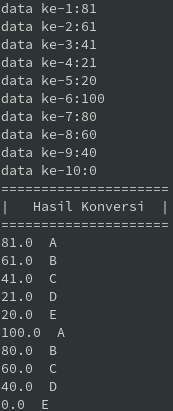
\includegraphics[scale=1]{8.png} 
\end{center}


\newpage

\section{Kesimpulan}
Setalah praktik mahasiswa dapat menyelesaikan kasus dengan menggabungkan konsep iterasi, seleksi dalam method serta dapat memanngil
method dari class lain.

\end{document}
